\subsection{Implementierung in C\#\hfill\textnormal{\emph{Walter}}}
Die Software wurde mithilfe von C\# implementiert, dies hat den Hintergrund, dass Unity diese Sprache verwendet. So konnte das ganze Projekt in einer Sprache einheitlich implementiert werden. 

C\# eignet sich durch seine Objekt orientiertheit sehr gut für die Beschreibung Komplexer Systeme. Jedes Objekt welches in dem behandelten Szenario vorhanden ist, wurde im Code implementiert. Die vorhandenen Klassen werden in einem Klassen-Diagramm in Abbildung \ref{ClassDiagram} illustriert.

Jede dieser Klassen hat verschiedene Methoden und Attribute. Die Objekte werden in Abschnitt \ref{obj} weiter erläutert. 

\subsubsection{Objekte}
\label{obj}
Die Simulation des Roboters sollte so genau wie möglich sein, daher wurden alle Gegenstände die mit dem Roboter Interagieren eigenständige Objekte. Bei den Objekten kann es sich um sogenannte Ground-Objekte handeln, welche jedes Objekt beschreiben, welches auf der Karte auftauchen kann. So erben Die Obstacle-Objekte von den Ground-Objekten die Position und das Traversable Attribut. Dies wird in Abbildung \ref{erben} illustriert. 

\begin{figure}[H]
  \centering{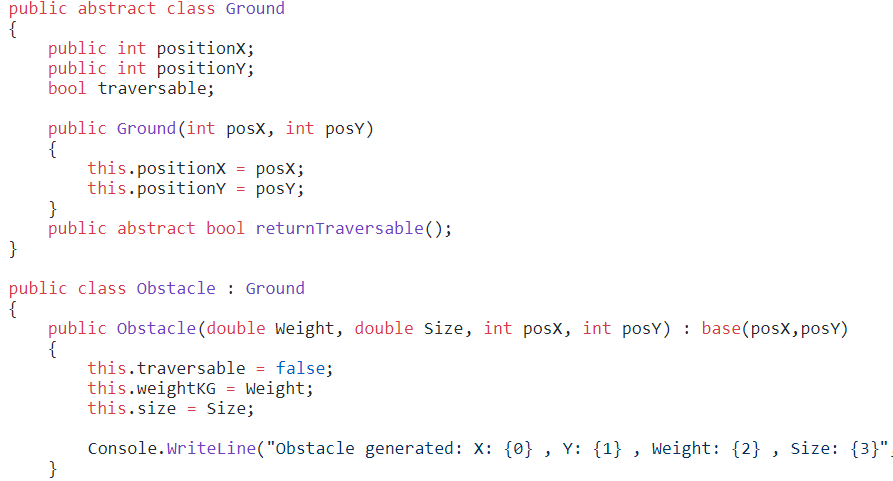
\includegraphics[width=1.0\linewidth]{Abbildungen/implementierung/vererbung.PNG}}
  \caption{Vererbung von Ground-Objekt zu Obstacle-Objekt}
  \label{erben}
\end{figure}
Zusätzlich zu den Ground-Objekten gibt es Peripherie Geräte für den Roboter, wie zum Beispiel die Kamera oder das Mikrophon. Auch Bauteile wie Motoren wurde mit verschiedenen Eigenschaften implementiert. So kann ein Motor zum Beispiel einen Namen, eine Anfangs- und End-position, eine Geschwindigkeit und einen State besitzen.

Die Rescue Bot Klasse, welche in Abbildung \ref{bot2} zu sehen ist, beinhaltet alle Sensoren und Aktoren, welche durch den Roboter miteinander interagieren. 

\begin{figure}[H]
  \centering{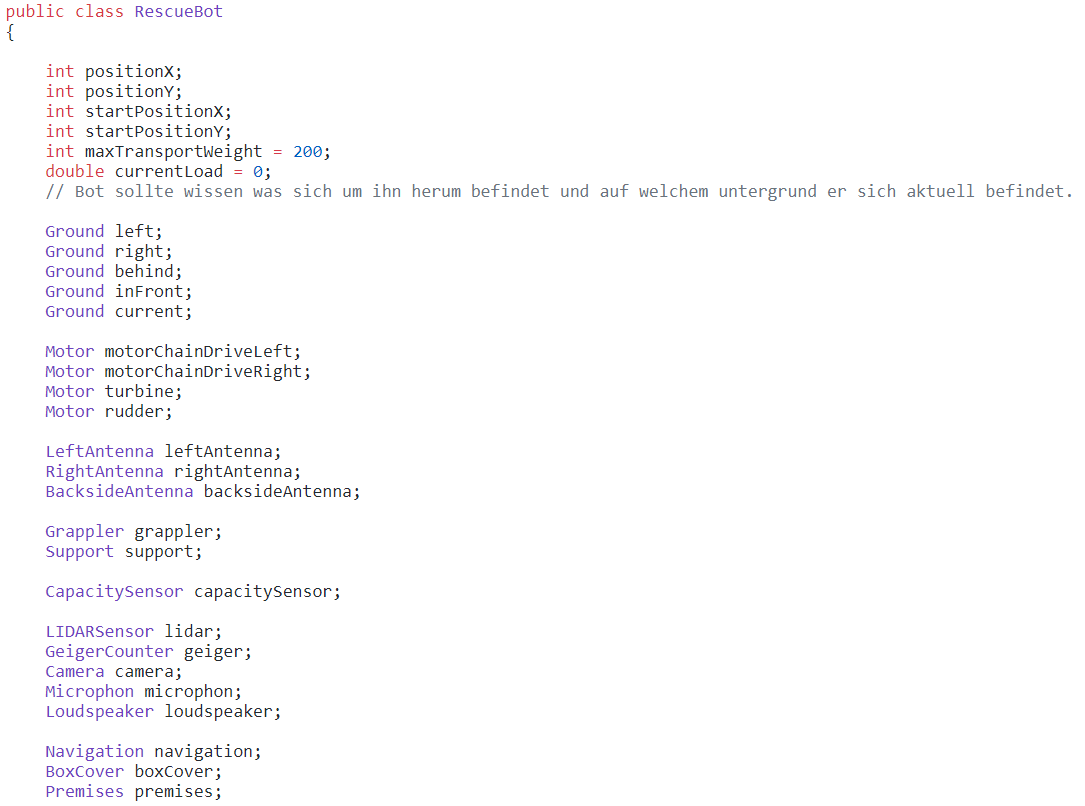
\includegraphics[width=1.0\linewidth]{Abbildungen/implementierung/rescueBotClass2.PNG}}
  \caption{Rescue Bot Klasse}
  \label{bot2}
\end{figure}
So befindet sich zum Beispiel der LIDAR Sensor, der Grappler und der Geigerzähler innerhalb der Rescue Bot Klasse. Durch diese Verkettung kann der Rescue Bot auf die Methoden der Geräte welche auch wieder Klassen sind zugreifen. 


\subsubsection{Karte}
\label{map}
Die Karte wird aus einem zweidimensionalen Array generiert. Das Eingabe Array besteht dabei aus verschieden Strings. Aus diesem Input wird mithilfe einer Switch-Case Anweisung ein neues Array generiert, welches aus Objekten besteht, die den Strings innerhalb des Eingabe Arrays entsprechen. Das Eingabe Array wird in Abbildung \ref{map} dargestellt. 

\begin{figure}[H]
  \centering{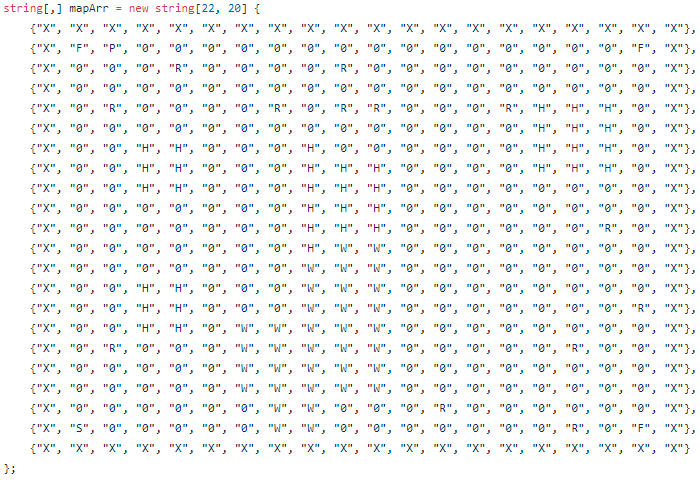
\includegraphics[width=1.0\linewidth]{Abbildungen/implementierung/mapArr.PNG}}
  \caption{Zweidiemensionales Array als Karte}
  \label{map}
\end{figure}

So wird zum Beispiel aus einem "R“ innerhalb des Eingabe Arrays ein Radioaktives Objekt erstellt, welches eine zufällige Größe, Gewicht und Strahlung als Attribute besitzt. Der Prozess der Objekt Instanziierung kann in Abbildung \ref{rad} betrachtet werden. 

Eine Aufschlüsselung der einzelnen Buchstaben und ihrer Bedeutung wird in Folgender Tabelle erläutert:
\begin{table}[H]
\centering
\begin{tabular}{l|l}
Zeichen & Bedeutung                 \\ 
\hline
0       & Frei befahrbarer Untergrund             \\
W       & Wasser                    \\
X       & Wand / Äußere Begrenzung  \\
S       & Startpunkt                \\
F       & Funkturm                  \\
R       & Radioaktives Objekt       \\
P       & Person  
\label{buchstaben}
\end{tabular}
\end{table}

Die Objekte werden direkt in das objArr Array gespeichert, was beispielhaft in der vorletzten Zeile in Abbildung \ref{map} zu sehen ist. 


\begin{figure}[H]
  \centering{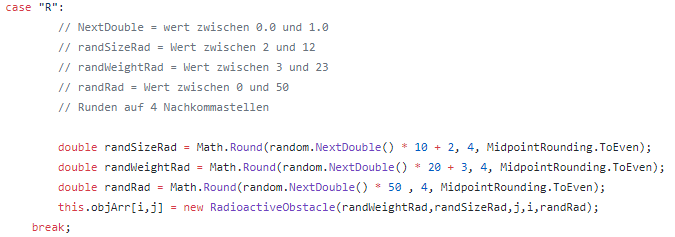
\includegraphics[width=1.0\linewidth]{Abbildungen/implementierung/createRadObj.PNG}}
  \caption{Instanziierung von Radioaktiven Objekten}
  \label{rad}
\end{figure}

\subsubsection{Erkennung und Bergen von Radioaktiven Gegenständen}
\label{erk}
Die Erkennung und das Bergen von Radioaktiven Gegenständen ist eins der Hauptfeatures des Rescue Bots. Die Erkennung der Objekte erfolgt in mehreren schritten. Bevor der Bot fährt wird über den LIDAR Sensor die unmittelbare Umgebung gescannt. Hierbei werden die Punkte vor, hinter, links, rechts und unter dem Bot erkannt. Felder welche Diagonal zum Bot liegen werden ignoriert. Sollte sich auf einem Feld welches direkt an den Bot grenzt ein Radioaktives Objekt liegen, wird dieses aufgesammelt wenn es bestimmten Kriterien entspricht. Die Kriterien sind, die Größe, die Abgegebene Radioaktive Strahlung und das Gewicht. 

Zu erst wird die Größe des Objektes mithilfe das LIDAR Sensors geprüft. Liegt das Objekt unterhalb der Maximalen Größe wird der Greifer in Richtung des Objektes bewegt und die Radioaktive Strahlung durch den Geigerzähler gemessen. Sollte die Strahlung einen Bestimmten Wert übersteigen wir das Objekt gegriffen und das Gewicht gemessen. Ist auch das Gewicht geringer als das maximale Gewicht, kann der Gegenstand bewegt eingesammelt werden. 

Dieser Prozess kann auch anhand des Aktivitätsdiagrams in Abbildung \ref{Rescue_object} nachvollzogen werden.
\subsubsection{Navigation}
\label{nav}
Der Bot soll Autonom durch eine generierte Karte fahren. Zur Hilfestellung gibt es innerhalb der Karte drei Funktürme. 

Jeder dieser Funktürme hat eine ID und eine Position auf der Karte. Diese Daten kann jeder der Funktürme an den Rescue Bot senden. Aus diesen Daten kann der Bot entscheiden welcher Funkturm der nächste ist und fährt in diese Richtung. 

Die Berechnung der Distanz wird in Abbildung \ref{dist} gezeigt. 
\begin{figure}[H]
  \centering{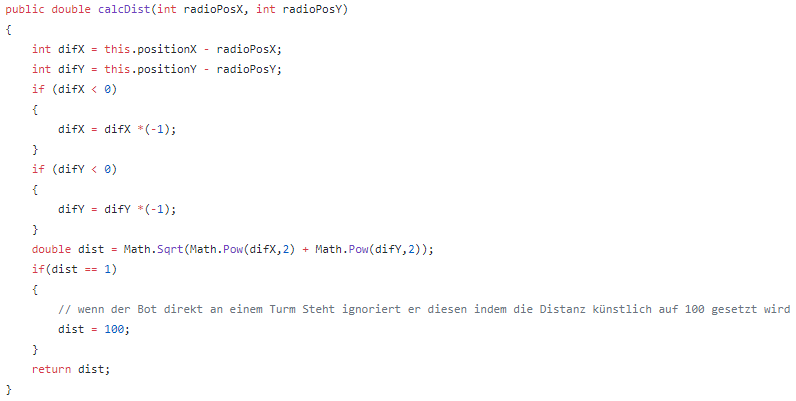
\includegraphics[width=1.0\linewidth]{Abbildungen/implementierung/calcDist.PNG}}
  \caption{Berechnung der Distanz zwischen zwei Punkten auf einer Fläche durch den Satz des Pythagoras}
  \label{dist}
\end{figure}

Entspricht die gemessene Distanz einer Längeneinheit (dist = 1), steht der Bot direkt neben dem Funkturm. Um den Funkturm für weitere Berechnungen zu ignorieren, wird die Distanz auf eine hohe Zahl gesetzt, im Beispiel in Abbildung \ref{dist} ist dies 100. Dies hat zur Folge, dass nun die Kürzeste Distanz zwischen den zwei verbleibenden Funktürmen gewählt wird.

Um sich zu den verschiedenen Funktürmen zu bewegen, können verschiedene Ansätze gewählt werden. 

In diesem Fall wird die Differenz der X- und Y-Koordinate berechnet und anschließend versucht die Differenz auf Null zu bringen. Dies geschieht indem zwischen einer Bewegung in X-Richtung und in Y-Richtung gewechselt wird, um eine Diagonale Bewegung zu ermöglichen. Auf diese Art und Weise kann die gefahrene Strecke minimiert werden. 

Sollten sich Hindernisse auf dem Weg befinden, versucht der Bot in eine zufällige Richtung auszuweichen und versucht es erneut, solange bis das Hindernis umfahren ist.

\subsubsection{Test Case}
\label{test}
Zum Testen des Systems wurde ein Szenario entwickelt, welches einige der Funktionen des Roboters überprüft. 

So soll getestet werden ob der Roboter den Rotor einschaltet, wenn er schwimmt, ob er Radioaktive Gegenstände eigenständig findet und einsammelt und ob einer eine Person erkennt und mit ihr interagiert. 

Folgende Einschränkungen wurden dabei festgelegt: 

\begin{itemize}
	\item Es gibt genau eine Person, welche sich an einem der in Abschnitt \ref{nav} beschriebenen Funktürme befinden muss
	\item Die Radioaktiven Gegenstände dürfen frei verteilt werden
	\item Hindernisse dürfen frei verteilt werden
	\item Es wird auf Sicht Einschränkungen durch Nebel verzichtet
	\item Bewegliche Hindernisse werden nicht berücksichtigt und entfernt
\end{itemize}
 
Das Ziel des Test Case ist, dass der Roboter So lange an Funktürmen nach einer Person sucht bis er sie gefunden hat. Während er auf der Suche ist, soll er jedes Radioaktive Objekt einsammeln, welches er findet, solange er nicht voll beladen ist. Außerdem soll angezeigt werden, welcher Motor aktuell verwendet wird.

Der Programmablauf ist als erfolgreich anzusehen, wenn die Person gefunden wurde und die Aktuelle Ladung ausgegeben wurde.

\begin{figure}[H]
  \centering{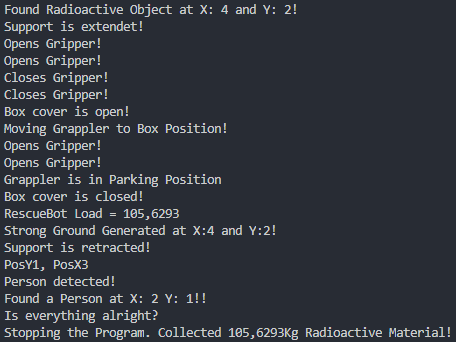
\includegraphics[width=1.0\linewidth]{Abbildungen/implementierung/output.PNG}}
  \caption{Ausgabe des Programms (Einsammeln von Radioaktiven Gegenständen und Interaktion mit Personen)}
  \label{output}
\end{figure}

\begin{figure}[H]
  \centering{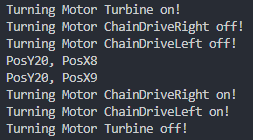
\includegraphics[width=1.0\linewidth]{Abbildungen/implementierung/waterr.PNG}}
  \caption{Ausgabe des Programms (Verwendung des Aktuellen Motors)}
  \label{waterr}
\end{figure}

Wie in Abbildung \ref{output} abgelesen werden kann, findet der Rescue Bot ein Radioaktives Objekt, Fährt den Greifer aus und entfernt es. Im weiteren Programmverlauf findet der Rescue Bot die Person und hat begonnen mit ihr zu interagieren. Somit ist das Einsammeln von Radioaktiven Gegenständen und die Interaktion mit Personen funktionsfähig. 

In Abbildung \ref{waterr} wird gezeigt welche Motoren aktuell verwendet werden und welche abgeschaltet sind. Fährt der Rescue Bot auf der Wasser Oberfläche so ist die Turbine aktiv, fährt er auf Land sind die Beiden Motoren für den Kettenantrieb aktiviert. Somit konnte auch diese Funktion validiert werden.